\documentclass[times,5p, twocolumn]{elsarticle}
\usepackage{parskip}
\begin{document}
\begin{frontmatter}
\title{LA INFORMÁTICA FORENSE EN DISPOSITIVOS ANDROID\\ }

\author{Farinango Yadira; Rodriguez Genith\\
}

\begin{abstract}
En este artículo se estudian los principales conceptos de la informática forense. Qué
es la informática forense, cuáles son sus objetivos y sus principios. También se mencionan
algunas técnicas anti-forenses, el manejo de la evidencia digital, los modelos forenses y la
legislación colombiana relacionada con la evidencia digital. Se hace énfasis en las buenas
prácticas para la realización de un análisis forense.

\textbf{Palabras clave:} Análisis forense digital móvil, Dispositivos Android, Estado del arte,
Informática forense.
\end{abstract}

\end{frontmatter}

\section{INTRODUCCIÓN}
\noindent
La evolución de los dispositivos móviles
ha aumentado considerablemente en los
últimos años, ha pasado de ser simples
celulares a computadores de mano. Por esta razón, las actividades cotidianas de las
personas como revisar correos
electrónicos, redes sociales, sitios de
interés, incluso la banca online, han pasado
a realizarse en dichos dispositivos. Éstos,
se han convertido en una extensión de la vida diaria de la personas, tanto personal
como laboralmente. 

Android sigue siendo la plataforma más
popular entre los usuario y también entre
los cibercriminales, siendo el principal
blanco entre todas las plataformas móviles.
Según Kaspersky Security Network, el
99 por ciento de las muestras de malware actuales
analizadas por dicho laboratorio de
seguridad están dirigidas a dispositivos
móviles se han desarrollado para esta
plataforma. También aclara que hay dos
razones principales por las que los
cibercriminales están interesados en
Android: su popularidad y su
funcionalidad (Kaspersky Lab, 2013).

\section{INFORMÁTICA FORENSE}
La computación o informática forense es
un área que se ha venido desarrollando
desde la última década del siglo XX. Esta
área es el resultado de una necesidad:
obtener una nueva fuente de material
probatorio. Las escenas criminales no solo
se limitaba a pruebas balísticas, muestras
de sangre, sino que también, los elementos
electrónicos podrían brindar pistas, ayudar
a formalizar una hipótesis y llevar a
resolver un caso judicial. 

Otra definición que puede describir lo que
es un análisis forense es: enfoque científico
que aprovecha efectos electromagnéticos
para «recolectar, analizar, verificar y
validar todo tipo de información existente,
o información que se considerada como
borrada» usando un conjunto de
herramientas y técnicas (Arias Chaves,
2006). Esta área, al tener un enfoque
científico cuenta con principios que rigen
la forma como se debe llevar dicho
análisis, para garantizar su veracidad e
integridad, ver Fig. 1. Para esta finalidad
se creó la IOCE (International
Organization of Computer Evidence)
(Rodríguez & Doménech, 2011).

\begin{figure}[h]
    \centering
    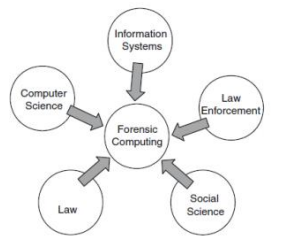
\includegraphics[width=5cm]{articulo.png}
    \caption{Dominio de la informática forense. } Fuente: (Broucek & Turner, 2006)
\end{figure}

\textbf{2.1. Técnicas anti-forenses}

Tradicionalmente las técnicas anti-forenses
se han clasificado en dos tipos: técnicas
anti-forenses transitorias y las técnicas
anti-forenses definitivas. En la técnica antiforense transitoria, se busca dificultar el
análisis con una herramienta o
procedimiento específico, pero no lo hace
imposible de analizar. Algunos ejemplos
son: fuzzing, abuso de los sistemas de
ficheros con el fin de crear mal
funcionamiento o para explotar
vulnerabilidades de las herramientas
usadas por el analista. La técnica antiforense definitiva va más allá, busca
arruinar las pruebas por lo que es
imposible adquirirlas. Algunos ejemplos
son: cifrado y borrado seguro (Maggi,
Zanero, & Iozzo, 2008).

Algunos de los objetivos que se busca
alcanzar con el uso de técnicas antiforenses son: limitar la detención de un
evento que ya ha ocurrido, distorsionar
información residente en el sitio,
incrementar tiempo requerido para
investigar el caso, generar dudas en
informe forense, engañar y limitar la
operación de herramientas forenses,
eliminar rastros que pudieron haber
quedado luego de los hechos realizados
(Álvarez & Guamán, 2008).

\textbf{2.2. Evidencia digital}

La evidencia digital o electrónica es
definida por el Instituto Nacional de tecnologías de la Comunicación de España
como todos aquellos datos que «de manera
digital se encuentran almacenados o fueron
transmitidos mediante equipos
informáticos y que son recolectados
mediante herramientas técnicas
especializadas empleadas por un perito en
una investigación informática». Cuya
funcionalidad es «servir como prueba
física (por encontrarse dentro de un
soporte) de carácter intangible (no
modificables) en las investigaciones
informáticas», Ver Fig. 2. 

\begin{figure}[h]
    \centering
    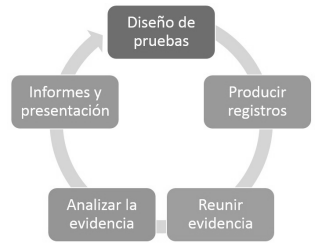
\includegraphics[width=5cm]{arti.png}
    \caption{Ciclo de la evidencia digital.  } Fuente: (Ghosh, 2004)
\end{figure}

La evidencia de sebe tomar en orden de
volatilidad, de la más volátil a la menos
volátil, en ese orden de ideas sería:

\begin{itemize}
    \item{Registros, caché} 
    \item{Tabla de enrutamiento, Caché ARP,
tabla de procesos, estadísticas del
kernel, memoria} 
    \item{Sistema de archivo temporales} 
    \item{Disco} 
    \item{Registro de datos y la monitorización
remota que sea relevante para el
sistema en cuestión} 
    \item{Configuración física, topología de
red} 
    \item{Los medios de comunicación de
archivos} 
\end{itemize}
\item 

\textbf{2.3. Modelos forenses}

Desde sus inicios hasta convertirse en una
ciencia, la informática forense sido descrita
por una serie de modelos que buscan guiar
este proceso. Estos modelos son similares,
varían en cuanto a algunas fases, unos más
detallados que otros.

El modelo de Casey ha evolucionado
desde su primera aparición en el 2000, que
consta de las siguientes fases (Casey ,
2011):

\begin{itemize}
    \item{Autorización y preparación} 
    \item{Identificación} 
    \item{Documentación, Adquisición y
Conservación} 
    \item{Extracción de información y Análisis} 
    \item{Reconstrucción} 
    \item{Publicación de conclusiones} 
\end{itemize}
\item 

\section{DISCUSIÓN }
La informática forense es un área de
mucha importancia y a su vez de mayor
cuidado. Para cumplir sus objetivos
interactúa con evidencia, que puede ser
presentada ante un juzgado para como
soporte probatorio, o también, a cualquier
empresa que solicite sus servicios para
resolver un problema interno. Alrededor de
la evidencia interactúan dos elementos
importantes: Las herramientas y el perito
informático. 

Estos temas se pueden trabajar a nivel
académico, usando herramientas con
licencias GPL, pero en un entorno laboral
se deben contar con las herramientas
hardware y software certificados por las
autoridades pertinentes. El perito
informático también debe certificar sus
conocimientos, no basta con ser bueno en
las ciencias computacionales. Cualquier
duda o error en estos dos puntos puede
poner en duda el soporte entregado por el
perito informático y por ende que el caso
se caiga.

\section{CONCLUSIONES}

La informática forense digital móvil es un
área interesante y de mucha relevancia en
el contexto actual. Con el crecimiento de
los peligros informáticos a la par del
mercado móvil, se abre un importante
camino investigativo y profesional.

Android, por su popularidad tanto para
clientes y cibercriminales, a la par de las
políticas actuales manejadas por Google
Inc. es unos de los sistemas operativos
móviles más interesante para trabajar. 

\section{REFERENCIAS}
Kaspersky Lab.  (2013).  \textit{Kaspersky Lab Latinoamérica.} Obtenido de http://latam.kaspersky.com/mx/sob
re-kaspersky/centro-deprensa/comunicados-deprensa/mC3A1s-de-la-mitadde-usuarios-de-android-no-pro

Arias Chaves, M. (2006).  \textit{Panorama
general de la informática forense y
de los delitos informáticos en Costa
RIca. InterSedes:} Revista de las
sedes regionales, VII(12), 141-154.

Rodríguez, F., & Doménech, A. (2011). \textit{ La
informática forense: el rastro digital
del crimen. Quadernos de
Criminología.} Revista de
Criminología y Ciencias
Forenses(14), 14-21.

Maggi, F., Zanero, S., & Iozzo, V. (2008).
\textit{ Seeing the invisible: Forensic Uses
of Anomaly Detection and
Machine Learning.} Newsletter, 42,
51-58.

Álvarez, M. D., & Guamán, V. A. (Febrero
de 2008). \textit{ Universidad Politécnica
Salesiana.} Obtenido de
http://dspace.ups.edu.ec/handle/123
456789/546

Casey , E. (2011). \textit{ Digital Evidence and
Computer Crime: Forensic
Science, Computers, and the
Internet (3rd ed.).} Academic Press.

\end{document} 